\section{PRISMA-2020-Guided Review Methodology}\label{sec:methodology}

To ground \texttt{RQ1} and parameterize the simulator from primary artifacts, I conducted a PRISMA-2020-guided literature review across Crossref, Semantic Scholar, OpenAlex, arXiv, ACM Digital Library, IEEE Xplore, USENIX, and official standards indices.

\subsection{Search Queries, Inclusion Criteria, and Screening}\label{subsec:prisma_search}
Candidate studies published between 2011 and November 2026 were retrieved across three channels, expanded in revision~v2 with targeted searches over 2024--November 2026 preprints and proceedings:
\begin{itemize}
    \item \textbf{Channel 1 (Carbon-Aware Cloud \& Serverless Scheduling, 16 records):} Paired carbon-intensity, grid emissions, SCI, and embodied terms with spatial/temporal shifting, serverless keep-alive, and cold-start mitigation (\texttt{Query A}).
    \item \textbf{Channel 2 (Phase-Disaggregated LLM Serving \& v2 Update, 44 records):} Combined LLM inference, KV caching, prefill/decode disaggregation, and GPU serving with energy, DVFS, power capping, and embodied/SCI queries (\texttt{Query B}, plus 2024--2026 arXiv/Crossref follow-ups on \texttt{"embodied carbon" AND "LLM" AND "inference"}, \texttt{"serverless" AND "keep-alive" AND "LLM" AND "carbon"}, \texttt{"Software Carbon Intensity" AND "LLM"}, and \texttt{"carbon-aware" + "prefill decode disaggregation"}). Exact boolean search strings and log dates appear in the online supplement.
    \item \textbf{Channel 3 (Surveys, Traces, Lifecycle Models \& Snowballing, 38 records):} Aggregated recent surveys, standards, hardware embodied datasets, citation chasing, and 9 systems verified during revision~v2~\cite{shi2024greenllm,topcu2026tension,sisodia2026sicp,zhang2026context,bernhard2026cleanest,tian2026greencache,moore2025slit,ozcan2025vidurvessim,nguyen2025sustainable}.
\end{itemize}

\textbf{Single-Author and AI-Assisted Screening Protocol:} All candidate retrieval, deduplication, and full-text eligibility checks were performed by a single human author assisted by generative AI search and extraction tooling; every included entry's bibliographic metadata, DOI/arXiv identifier, and quantitative metrics were verified directly against primary PDFs, HTML preprints, or Crossref records. As shown in Fig.~\ref{fig:prisma}, removing 3 duplicates from 98 identified records left 95 unique records for title/abstract screening. Excluding 14 out-of-scope records (lacking cloud serving, datacenter energy, or carbon context, including 3 edge/mobile/satellite works) yielded 81 candidates for eligibility assessment, where 20 more were excluded (offline training only, latency-only disaggregation/pruning, or superseded position notes), leaving 61 included works.

\begin{figure}[t]
    \centering
    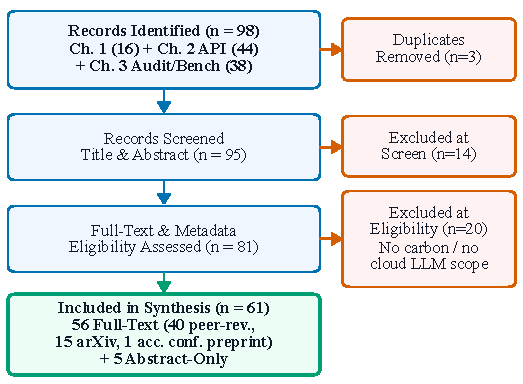
\includegraphics[width=\ifdefined\BUILDELSEVIER 0.85\linewidth\else 0.78\linewidth\fi]{figures/fig2_prisma_flow.pdf}
    \caption{PRISMA-2020-guided search, screening, and eligibility pipeline yielding the 61-work corpus (56 full-text, 5 abstract-only).}
    \label{fig:prisma}
\end{figure}

\subsection{Corpus Provenance and Preprint Disclosure}\label{subsec:corpus_audit}
The 61-work corpus comprises 47 empirical/modeling systems, 11 surveys or research agendas, 2 standards (ISO/IEC 21031:2024~\cite{iso2024sci} and NIST SP 800-145~\cite{mell2011nist}), and 1 trace release~\cite{azure2024trace}. By recency, 56/61 works (91.8\%) appeared in 2022--2026, and 34/61 (55.7\%) appeared in 2025--2026. Retrieval depth breaks down as:
\begin{enumerate}
    \item \textbf{Full-Text Audited (56/61, 91.8\%):} Complete texts underwent equation and table verification, spanning 40 archival publications/standards/traces plus 16 preprints (15 arXiv-only preprints~\cite{hewage2026carbon,yang2025container,pan2025inference,li2025ecoserve,basit2026dualscale,shi2024greenllm,topcu2026tension,sisodia2026sicp,zhang2026context,bernhard2026cleanest,ozcan2025vidurvessim,yan2026pdprov,jegham2025hungryai,zhen2025taming,lu2026etcinfer} and 1 accepted SIGOPS ATC 2026 preprint~\cite{wang2026festina}).
    \item \textbf{Abstract-Only Verified (5/61, 8.2\%):} Five paywalled records relied strictly on verified abstracts~\cite{roy2026lowcarb,calavaro2026offloading,gupta2022act,sinha2025utilization,calheiros2011cloudsim}, with zero constants imported into the simulator.
\end{enumerate}
